\section*{\large{ПРИЛОЖЕНИЯ}}
\addcontentsline{toc}{section}{ПРИЛОЖЕНИЯ}
\label{appendix}

\renewcommand{\thefigure}{\arabic{figure}}

\setcounter{figure}{0}

\lstset{
    string=[s]{"}{"},
    stringstyle=\color{blue},
    comment=[l]{:},
    commentstyle=\color{black},
    basicstyle=\footnotesize
}
\subsection*{\large{Приложение A. API сервисов}}
\addcontentsline{toc}{subsection}{Приложение A. API сервисов}
\begin{figure}[H]
	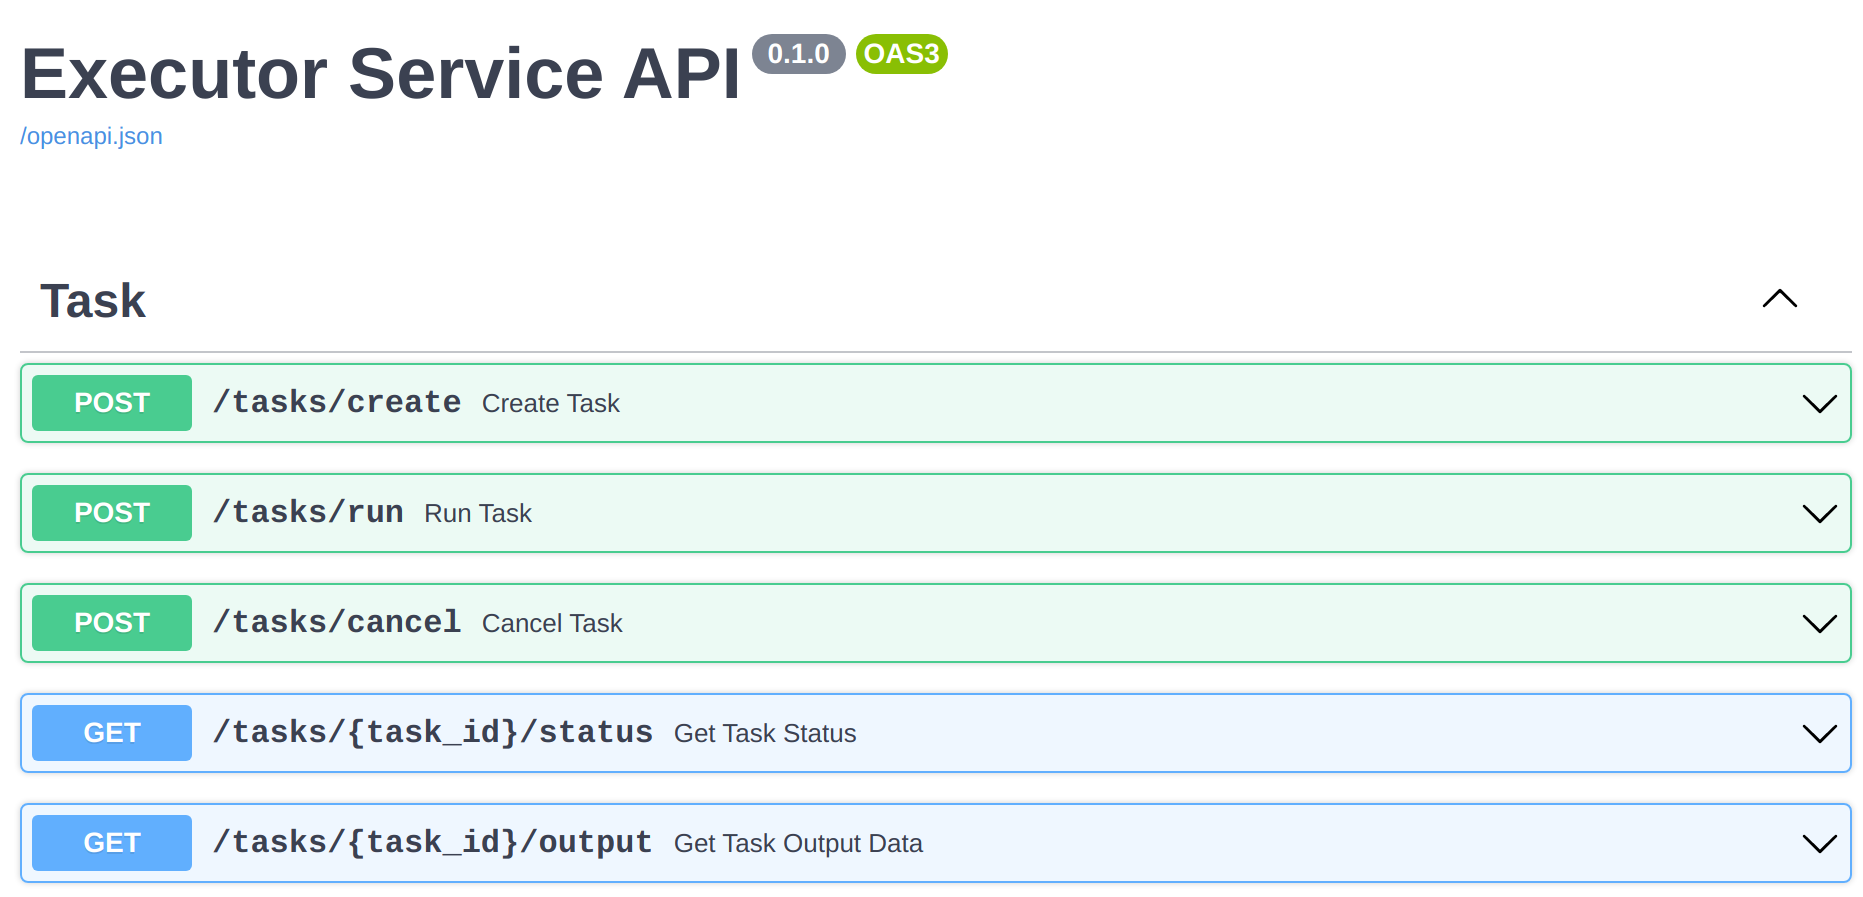
\includegraphics[width=\textwidth]{applications/pictures/executor_swagger}
	\caption{API сервиса запуска математических методов}
	\label{pic:application__executor-swagger}
\end{figure}
\vskip 10 mm
\begin{figure}[H]
	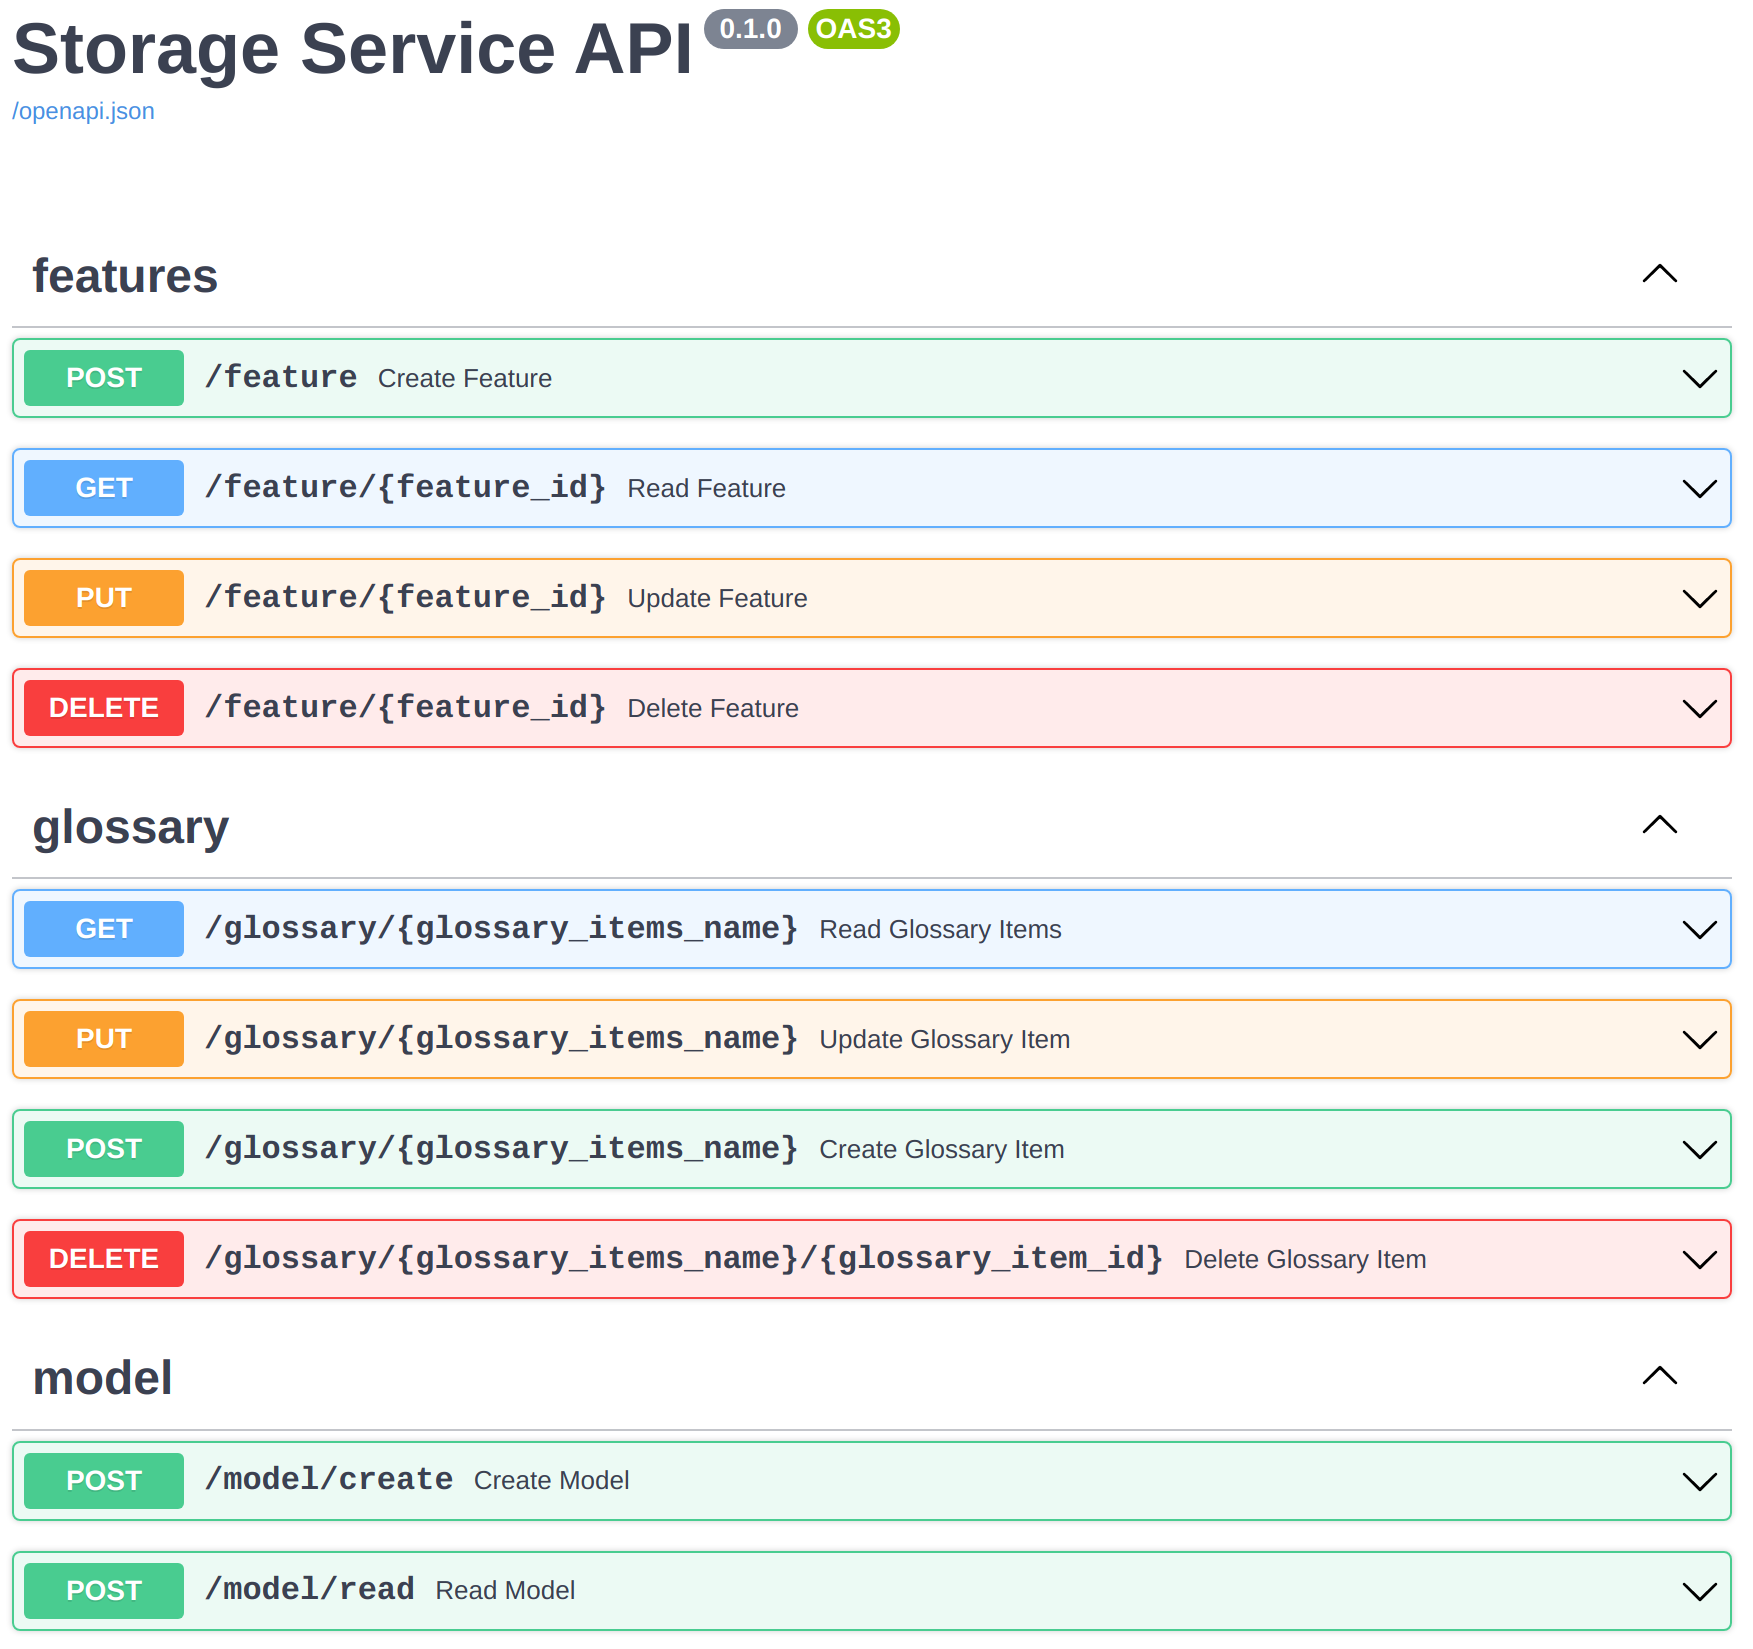
\includegraphics[width=\textwidth]{applications/pictures/storage_swagger}
	\caption{API сервиса хранения расчётных данных}
	\label{pic:application__storage-swagger}
\end{figure}
\vskip 10 mm
\begin{figure}[H]
	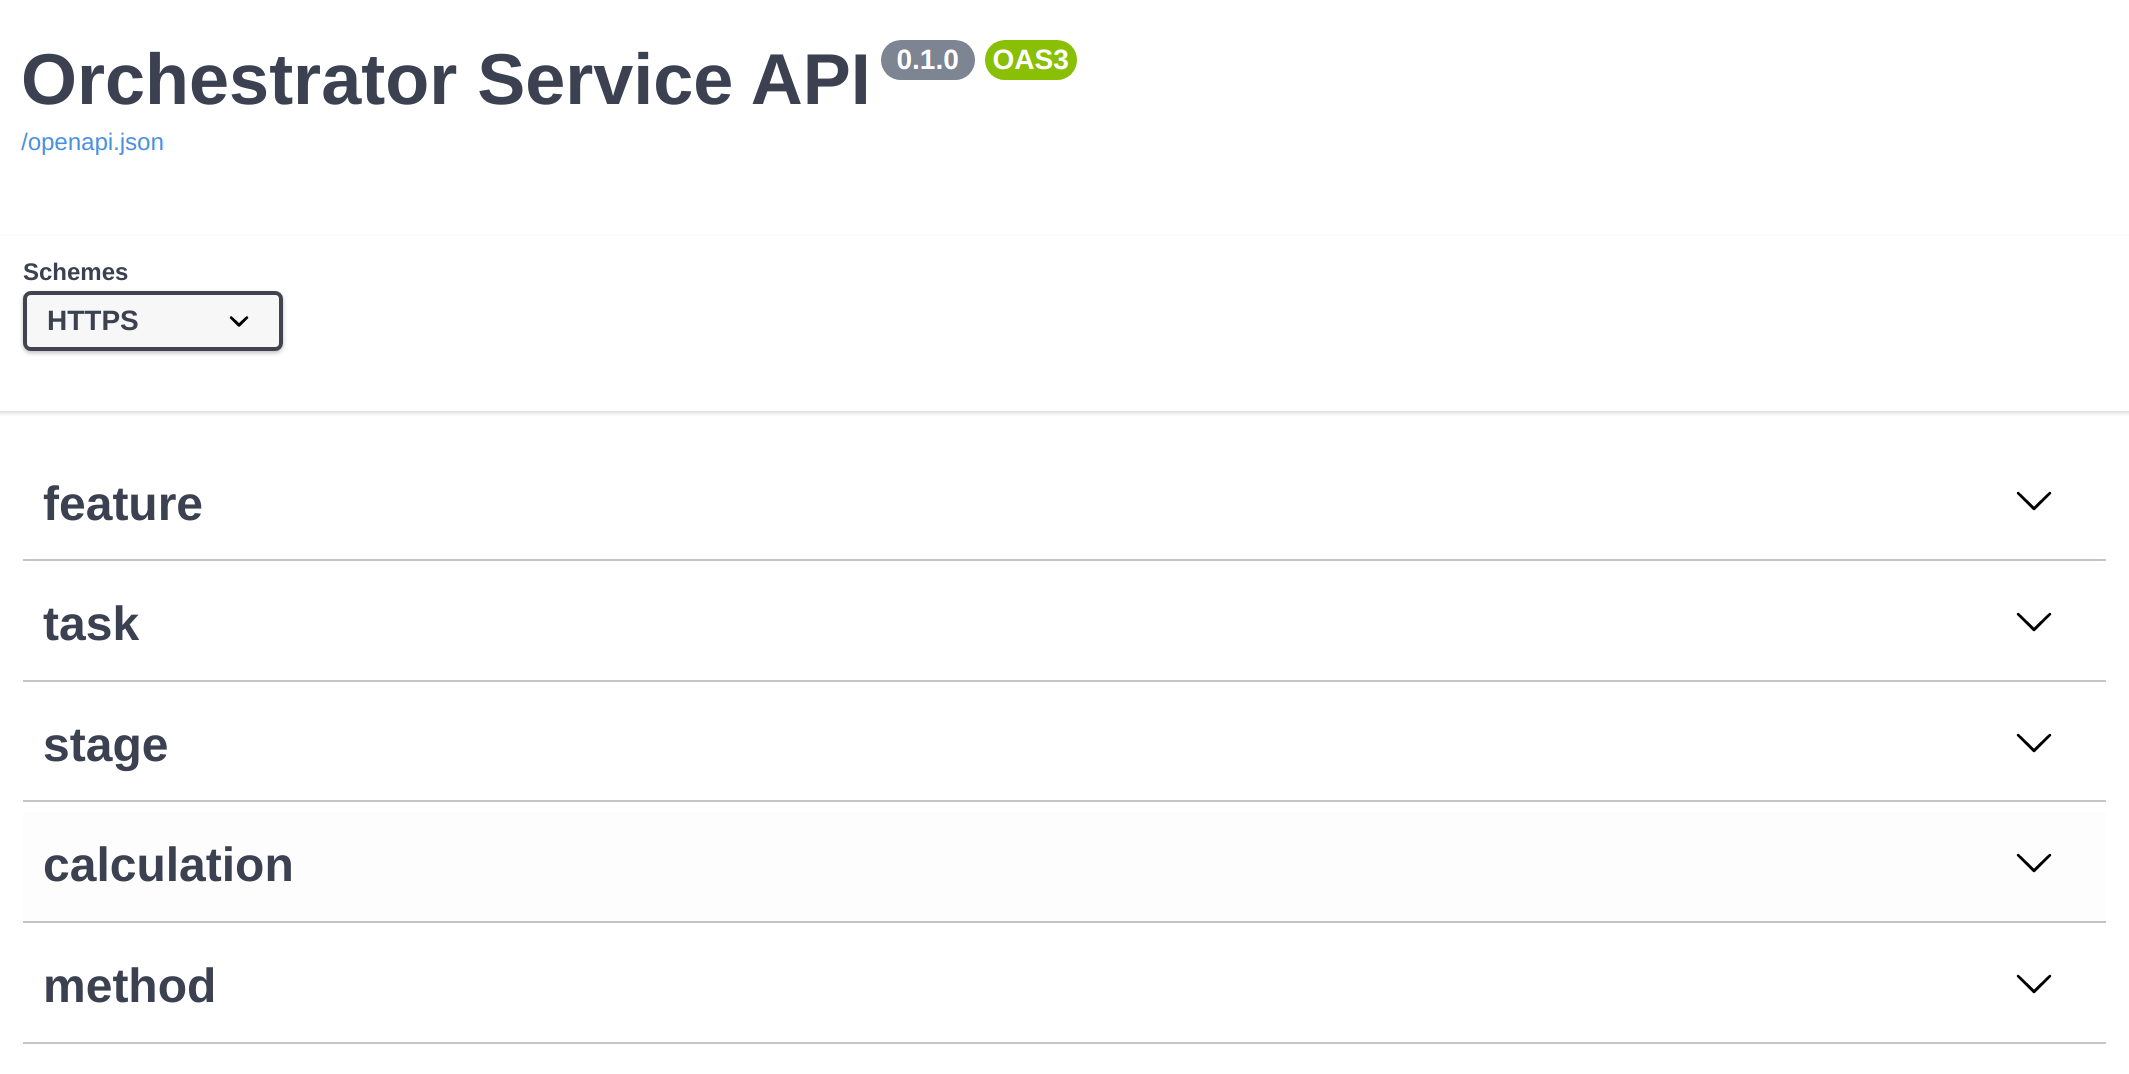
\includegraphics[width=\textwidth]{applications/pictures/orchestrator_swagger}
	\caption{API сервиса запуска расчётных задач}
	\label{pic:application__orchestrator-swagger}
\end{figure}
\vskip 10 mm


\subsection*{\large{Приложение Б. Фрагменты пользовательского интерфейса}}
\addcontentsline{toc}{subsection}{Приложение Б. Фрагменты пользовательского интерфейса}
\renewcommand{\thefigure}{\arabic{figure}}
\setcounter{figure}{0}

\begin{figure}[H]
	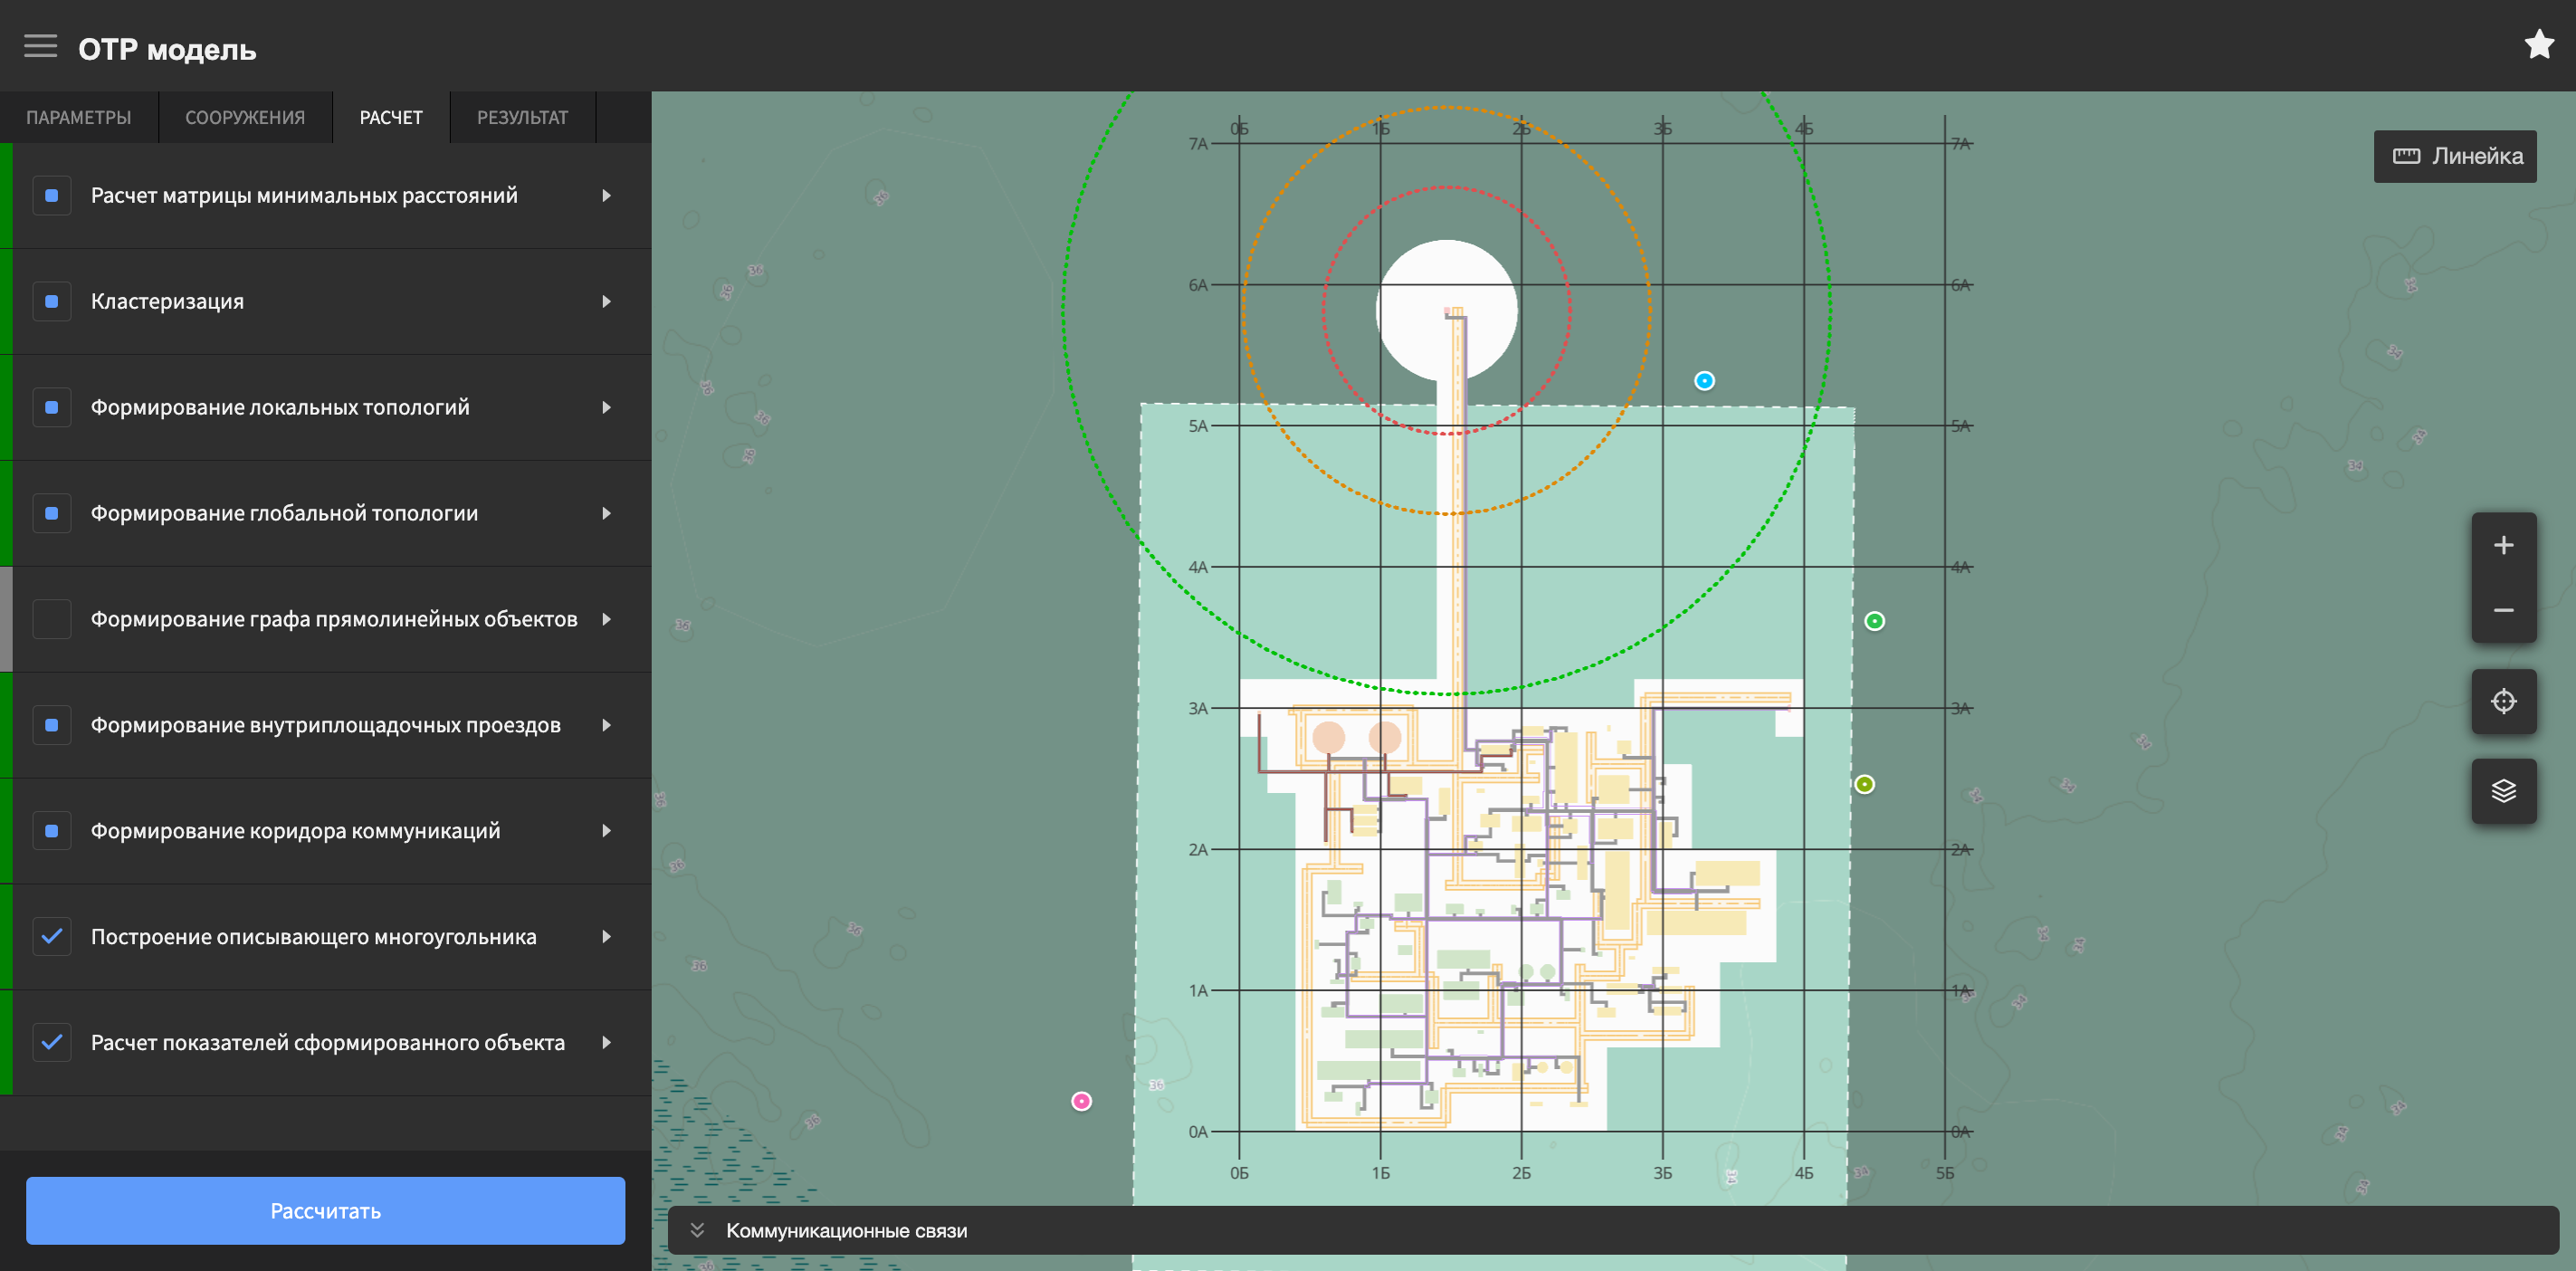
\includegraphics[width=0.68\textwidth]{applications/pictures/system}
	\caption{Скриншот интерфейса системы}
	\label{pic:application__system}
\end{figure}
\vskip 10 mm